\documentclass[12pt]{article}
\usepackage[utf8]{inputenc}
\usepackage{graphicx}
\usepackage{framed, color}
\usepackage{paralist, blindtext}

\definecolor{shadecolor}{rgb}{0.83,1,0.8}
\begin{document}

\begin{titlepage}

\newcommand{\HRule}{\rule{\linewidth}{0.5mm}} % Defines a new command for the horizontal lines, change thickness here

\center % Center everything on the page
 
%----------------------------------------------------------------------------------------
%	HEADING SECTIONS
%----------------------------------------------------------------------------------------

\textsc{\LARGE Universidad de Concepción}\\[1.5cm] % Name of your university/college
\textsc{\Large Departamento de Ingeniería Civil Informática y Ciencias de la Computación}\\[0.5cm] % Major heading such as course name
\textsc{\large Ingeniería de Software I}\\[0.5cm] % Minor heading such as course title

%----------------------------------------------------------------------------------------
%	TITLE SECTION
%----------------------------------------------------------------------------------------

\HRule \\[0.4cm]
{ \huge \bfseries Aplicación Movil en Apoyo al Turismo en la Provincia de Arauco }\\[0.4cm] % Title of your document
\HRule \\[1.5cm]
 
%----------------------------------------------------------------------------------------
%	AUTHOR SECTION
%----------------------------------------------------------------------------------------

\begin{minipage}{0.4\textwidth}
\begin{flushleft} \large
\emph{Author:}\\
Cristobal \textsc{Donoso}
Matías \textsc{Medina}\\
Diego \textsc{Rodriguez}
Meraioth \textsc{Ulloa}
\end{flushleft}
\end{minipage}
~
\begin{minipage}{0.4\textwidth}
\begin{flushright} \large
\emph{Supervisor:} \\
Gonzalo \textsc{Rojas} % Supervisor's Name
\end{flushright}
\end{minipage}\\[4cm]

{\large \today}\\[3cm] % Date, change the \today to a set date if you want to be precise
\vfill % Fill the rest of the page with whitespace
\end{titlepage}

%----------------------------------------------------------------------------------------
%	INTRODUCTION
%----------------------------------------------------------------------------------------
\section{Introducción}
Chile, por su geografía y diversidad climática, posee muchos lugares turísticos que yacen en el ojo de los que viajan. Sin embargo, actualmente existen lugares a pocos kilómetros de la ciudad, accesibles pero alejados en popularidad, como lo es la provincia de Arauco. Hemos escogido esta provincia dado que posee un valor cualitativo importante en el área del turismo (considerándola como una de las mayores fuentes de ingreso para la provincia) ocasionando un trade-off con el creciente avance de la gran industria.\\\\En este proyecto realizaremos un prototipo de solución el cual consiste en la creación de una aplicación móvil que ayude en la difusión, orientación y elección de puntos de interés para el turista. Se espera que esta aplicación pueda entregar un apoyo real hacia las pequeñas empresas que se encuentran registradas en el SERNATUR.\\\\Nuestra dinámica de trabajo funda sus bases en el \textbf{modelo de procesos tipo cascada} que, entre otras cosas, se caracteriza por separar las distintas fases de especificación e implementación de manera secuencial y sin retorno. Los procesos involucrados se relacionan con:
\begin{enumerate}
\item \textbf{Requerimientos}
\item \textbf{Diseño del Software} 
\item \textbf{Implementación y Testeo}
\item \textbf{Integración}
\item \textbf{Operación y Mantenimiento} 
\end{enumerate}  
\newpage
\section{Disciplinas de RUP para la iteración}
\subsection{Modelado del Negocio}
Se requiere un sistema computacional que permita facilitar el acceso a los servicios turísticos provistos por pequeños empresarios en la provincia de Arauco. Para ello se necesita almacenar en una base de datos los distintos servicios ofrecidos por los empresarios, la cual obtendrá parte de su información desde una base de datos proporcionada por SERNATUR.\\\\
Esta información será accedida desde una aplicación móvil, donde los usuarios podrán visualizar distintos puntos de interés, ya sean lugares de libre acceso o servicios ofrecidos por empresarios. Además el usuario podrá calificar los lugares que visita y crear itinerarios con distintos lugares para luego compartirlo.\\\\
Por otro lado, la aplicación tendrá integración de servicios como Google Maps para obtener rutas y redes sociales para compartir los lugares visitados.
\subsection{Requerimientos}
A partir del enunciado del problema extrajimos los distintos requerimientos que debe cumplir el sistema, éstos son:
\begin{enumerate}
\item Mantener información de servicios turísticos.
\item Obtener información desde los proveedores de servicios.
\item Enriquecer información por experiencia de turistas.
\item Busqueda de servicios registrados.
\item Evaluación de usarios a servicios.
\item Categorización de servicios.
\item Rutas a servicios.
\item Facilitar indicaciones a lugares de dificil acceso.
\item Indicaciones con fotografías de hitos y referencias conocidas.
\item Información de buses.
\item Proveer mapa temático de oferta turística.
\item Crear Itinerario.
\item Consultar itinerario.
\item Comentar itinerario.
\item Recomendaciones de itinerario para distinta duración.
\end{enumerate}
\subsection{Análisis y Diseño	} 
De los requerimientos previamente listados, se ha elaborado el siguiente diagrama de casos de uso, el cual muestra cuales son los actores involucrados en el sistema y los distintos casos de uso que éstos pueden llevar a cabo.
\begin{center}\begin{figure}[htp]
\centering
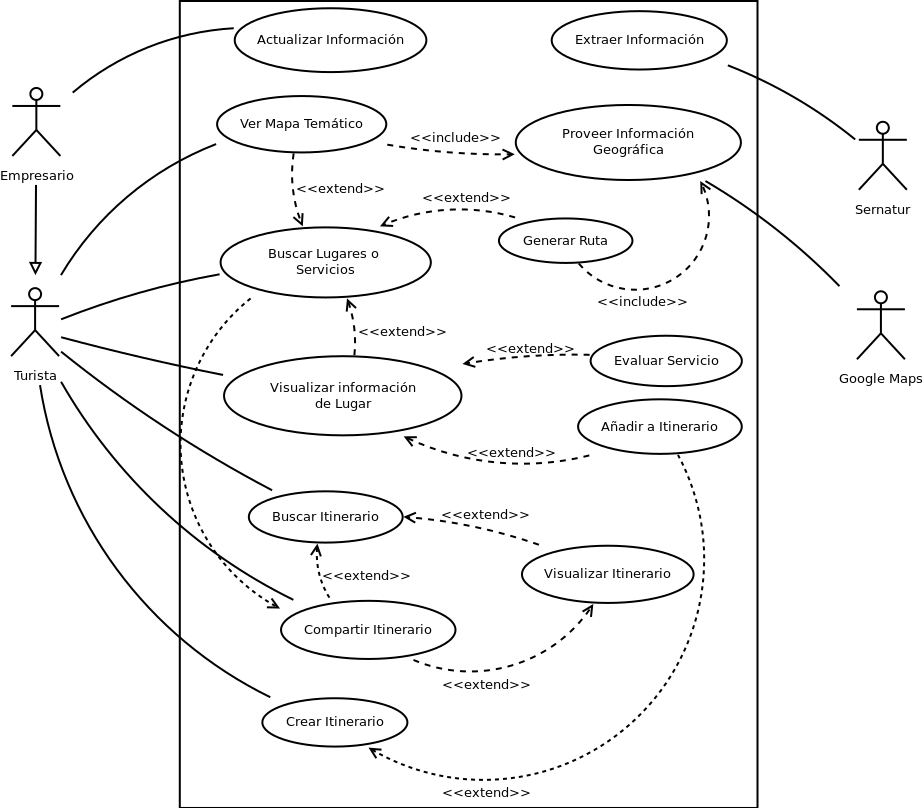
\includegraphics[scale=0.4]{Diagrama1.png}
\caption{Diagrama de Casos de Uso}
\label{}
\end{figure} \end{center} 
\newpage
\subsubsection{Documentación Casos de Uso}
Previo a definir los distintos casos de uso, es necesario definir algunos conceptos que servirán de guía para la documentación.
\paragraph{Glosario}
\begin{itemize}
\item \textbf{Categoría}: Clasificación  de una Sucursal según los servicios que presta.
\item \textbf{Empresario}: Representante legal de una sucursal.

\item \textbf{Empresa}: Organización que desarrolla una actividad turística

\item \textbf{Itinerario}: Conjunto de Lugares y/o Servicios ordenados y definidos por un usuario.

\item \textbf{Mapa Temático}: Mapa físico de la provincia que incluye iconos de lugares y servicios.

\item \textbf{Punto de interés}: Ubicación especifica en el mapa. 

\item \textbf{Ruta}: Secuencia de puntos que describe la mejor trayectoria entre dos lugares.

\item \textbf{Servicio}: Función(es) que desarrolla una sucursal.

\item \textbf{Sucursal}: Lugar turístico de una Empresa\\\\
\end{itemize}
%caso de uso ver mapa tematico
\underline{Caso de Uso:} \textbf{Ver mapa temático}\\\\\underline{Actor Principal}: Turista\\\\\underline{Personal involucrado e intereses}\\Turista: Quiere visualizar mapa de servicios de la provincia de Arauco.\\
Maps: Quiere recibir peticiones de PoI para mostrar en mapa de forma correcta.\\\\\underline{Precondiciones:} El sistema asigna a cada servicio un símbolo PoI.
Maps se encuentra conectado al sistema principal.\\\\\underline{Postcondiciones}: El turista visualiza un mapa ( geográfico) con marcas dónde aparecen el o los servicios que fueron seleccionados.\\\\\underline{Escenario principal de éxito:}
\begin{enumerate}
\item Se envía petición a Maps para proveer el mapa geográfico de la provincia de Arauco.
\item El turista visualiza el mapa geográfico de la provincia de Arauco.
\item El turista selecciona el o los servicios que desea visualizar en el mapa temático.
\item Se envía la petición a Maps para que provea el o los servicios (PoI) ubicados geográficamente.
\item Los servicios aparecen en el mapa geográfico según la símbolos PoI predefinidos.
\end{enumerate}
\underline{Extensiones:}
\begin{enumerate}
\item [1’] Falla la conexión con Maps , se muestra una alerta.
\item [4’] Falla la conexión con Maps , se muestra una alerta  y vuelve al paso 1.
\end{enumerate}
%caso de uso proveer informacion geografica
\underline{Caso de Uso:} \textbf{Proveer Información Geográfica} \\\\\underline{Actor Principal}: Maps\\\\\underline{Personal involucrado e intereses}\\Maps: Quiere recibir peticiones de información geográfica para enviar.\\\\\underline{Precondiciones:} Maps se encuentra conectado al sistema principal.\\\\\underline{Postcondiciones}: Maps entrega la información geográfica (mapa o POI).\\\\\underline{Escenario principal de éxito:}
\begin{enumerate}
\item Maps recibe petición para mostrar un mapa geográfico o puntos de interés.
\item Maps entrega mapa geográfico o puntos de interés.
\end{enumerate}
\underline{Extensiones:}
\begin{itemize}
\item[1'] Falla la conexión con Maps , se muestra una alerta.
\end{itemize}
%CASO DE USO GENERAR RUTA
\underline{Caso de Uso}: \textbf{Generar Ruta}\\\\
\underline{Actor Principal}: Google Maps\\\\
\underline{Personal Involucrado e Intereses}: Turista: Quiere encontrar la ruta optima entre el lugar seleccionado y su posición.\\Maps: Quiere recibir dos puntos geográficos para emitir un mapa geográfico con la ruta optima.\\\\
\underline{Precondiciones}:
\begin{itemize}
\item Maps se encuentra conectado al sistema principal.
\item Turista seleccionó un lugar ( donde se presta o no un servicio) de interés.
\item Turista sabe que medio de transporte utilizará.
\end{itemize}
\underline{Postcondiciones}: Se entrega un mapa junto a las indicaciones para llegar al lugar deseado.\\\\
\underline{Escenario principal de éxito}:
\begin{enumerate}
\item Se envía la información a Maps del punto de inicio y el punto final y el medio de transporte a utilizar.
\item Maps entrega mapa geográfico con una ruta ( trazo de carretera o camino) marcado identificando variantes del camino optimo según el medio de transporte.
\end{enumerate}
\underline{Extensiones}:
\begin{enumerate}
\item[1'] Falla la conexión con Maps , se muestra una alerta .
\item[2'] No existe ruta entre el punto de inicio y el punto de partida de acuerdo al medio de transporte a utilizar , se muestra una alerta y se inicia el caso de uso “Buscar Lugar o Servicio”.
\end{enumerate}
%CASO DE USO ACTUALIZAR INFORMACION
\underline{Caso de uso}: \textbf{Actualizar Información}\\\\
\underline{Actor Principal}: Empresario\\\\
\underline{Personal involucrado e intereses}: Empresario: Quiere Actualizar la información que se encuentra en la base de datos del Sistema.\\
Sistema: Quiere recibir información para agregar en la base de datos.\\\\
\underline{Precondiciones}: Se debe haber creado la base de datos con información recolectada desde el SERNATUR.\\\\
\underline{Postcondiciones}: La base de Datos del sistema queda actualizada con la nueva información.
\underline{Escenario principal de éxito}
\begin{enumerate}
\item El usuario agrega/borra información en la base de datos.
\item El sistema da cuenta de la modificación y actualiza la base de datos.
\end{enumerate}
\underline{Extensiones}
\begin{enumerate}
\item[1'- 2'] Cancelar: En cualquier momento el Empresario puede cancelar la operación.
\end{enumerate}
%CASO DE USO BUSCAR LUGARES O SERVICIO
\underline{Caso de uso}: \textbf{Buscar lugares o servicios}.\\\\
\underline{Actor Principal}: Turista\\\\
\underline{Personal involucrado e intereses}: Turista: Quiere encontrar un lugar determinado, o encontrar un lugar que cumpla sus expectativas.\\\\
\underline{Postcondiciones}: El turista obtiene una lista de los puntos de interés que cumplen con el criterio de búsqueda utilizado. Ya sea por nombre, tipo de servicio, calificación, etc.\\\\
\underline{Escenario principal de éxito}
\begin{enumerate}
\item El turista selecciona la opción de buscar y el criterio de búsqueda.
\item El sistema busca en la base de datos los puntos de interés que cumplan los requisitos del turista.
\item El sistema despliega en la pantalla los puntos de interés que cumplen con la búsqueda.
\end{enumerate}
\underline{Extensiones}
\begin{enumerate}
\item[1'] Si desea buscar por nombre, debe ingresar la palabra que quiere buscar.
\item[2'] Si el sistema no encuentra lugares que cumplan los criterios de búsqueda entonces despliega en pantalla que no existen coincidencias con la búsqueda.
\end{enumerate}
%CASO DE USO EVALUAR SERVICIO
\underline{Caso de uso}: \textbf{Evaluar servicio}.\\\\
\underline{Actor Principal}: Turista.\\\\
\underline{Personal involucrado e intereses}: Turista: Quiere darle una calificación al servicio que utilizó, o dar su opinión sobre él.\\\\
\underline{Precondiciones}: El turista debe estar visualizando la información del lugar (Caso de Uso: Visualizar información del lugar).\\\\
\underline{Postcondiciones}: El turista agrega a la base de datos del sistema la puntuación asociada a ese servicio y/o un comentario acerca de su experiencia para que los demás usuarios puedan ver esta información.\\\\
\underline{Escenario Principal de Éxito}:
\begin{enumerate}
\item El turista selecciona un criterio de calificación y califica con estrellas el servicio (una a cinco).
\end{enumerate}
\underline{Extensiones}
\begin{enumerate}
\item[1'a] Puede volver a evaluar según tantos criterios como quiera.
\item[1'b] Si lo desea puede agregar comentarios escritos en un espacio designado para escribir texto. 
\end{enumerate}
%CASO DE USO CREAR ITINERARIO
\underline{Caso de uso}: \textbf{Crear itinerario}\\\\
\underline{Actor Principal}: Turista\\\\
\underline{Personal involucrado e intereses}: Turista: Quiere crear un itinerario dentro de la aplicación.\\\\
\underline{Precondiciones}: El turista, desde sus itinerarios, accede a la creación de itinerario.\\\\
\underline{Postcondiciones}: El turista crea un itinerario vacío.\\\\
\underline{Escenario principal de éxito}:
\begin{enumerate}
\item El Turista escribe el nombre del nuevo itinerario.
\item Si el nombre no se repite con otro itinerario del usuario, se crea el nuevo itinerario.
\end{enumerate}
\underline{Extensiones}:
\begin{enumerate}
\item[1-2'] Cancelar: En cualquier momento el Turista puede cancelar la operación. 
\item[2'] El nombre del itinerario ya existe: Se emite un mensaje y se vuelve al paso 1.
\end{enumerate}
%CASO DE USO AÑADIR LUGAR A ITINERARIO
\underline{Caso de uso}: \textbf{Añadir lugar a itinerario}\\\\
\underline{Actor Principal}: Turista.\\\\
\underline{Personal involucrado e intereses}: Turista: Quiere agregar un lugar a un itinerario creado por él con anterioridad.\\\\
\underline{Precondiciones}:  Se debe haber estado en la parte de visualización de un lugar específico.\\\\
\underline{Postcondiciones}: El turista agrega un lugar a un itinerario específico.\\\\
\underline{Escenario principal de éxito}:
\begin{enumerate}
\item El turista selecciona opción para agregar el lugar al itinerario.
\item El turista selecciona el itinerario al cual quiere agregar el lugar.
\item Si el lugar no era el último dentro del itinerario, este se agrega al final del itinerario
\end{enumerate}
\underline{Extensiones}:
\begin{enumerate}
\item[2-3'] Cancelar:En cualquier momento el Turista puede cancelar la operación. 
\item[3'] El lugar se encontraba en la última posición del itinerario: Se emite un mensaje y se vuelve al paso 2.
\end{enumerate}
%CASO DE USO BUSCAR ITINERARIO
\underline{Caso de uso}: \textbf{Buscar itinerario}\\\\
\underline{Actor Principal}: Turista\\\\
\underline{Personal involucrado e intereses}: Turista: Quiere encontrar un itinerario determinado, o encontrar un itinerarios que cumplan una serie de criterios de búsqueda.\\\\
\underline{Precondiciones}:  El turista está visualizando una lista con todos los itinerarios disponibles.\\\\
\underline{Postcondiciones}: El turista obtiene una lista de los itinerarios que cumplen con el criterio de búsqueda utilizado. Ya sea por nombre, lugares y servicios contenidos, etc.\\\\
\underline{Escenario principal de éxito}
\begin{enumerate}
\item El turista selecciona la opción de búsqueda.
\item El turista ingresa palabra clave.
\item El sistema busca en la base de datos los itinerarios que cumplan los criterios del turista.
\item Si la búsqueda fue realizada con éxito, el sistema despliega en la pantalla los itinerarios encontrados.
\end{enumerate}
\underline{Extensiones}
\begin{enumerate}
\item[2'a] Cancelar: El turista puede decidir no llevar a cabo la búsqueda.
\item[2'b] Se puede agregar algún criterio de búsqueda adicional, de tipo localidad, lugar, servicio, etc.
\item[4'] La búsqueda no entregó ningún resultado: Se emite un mensaje y se vuelve al paso 2.
\end{enumerate}
%CASO DE USO COMPARTIR ITINERARIO
\underline{Caso de uso}: \textbf{Compartir itinerario}\\\\
\underline{Actor Principal}: Turista\\\\
\underline{Personal involucrado e intereses}: Turista: Quiere compartir un itinerario de su interés en las redes sociales.\\\\
\underline{Precondiciones}: Se debe estar dentro de la visualización de un itinerario especifico.\\\\
\underline{Postcondiciones}: El itinerario es compartido exitosamente en la red social elegida por el usuario.\\\\
\underline{Escenario principal de éxito}
\begin{enumerate}
\item El turista selecciona la opción de compartir.
\item El turista selecciona la red social.
\item El turista envía la solicitud a la red social.
\item Si la solicitud fue realizada con éxito se avisa al turista.
\end{enumerate}
\underline{Extensiones}:
\begin{enumerate}
\item[2'] Cancelar: El turista puede decidir no compartir el itinerario.
\item[4'] La solicitud fue rechazada por la red social: Se emite un mensaje y se vuelve al paso 2.
\end{enumerate}
%CASO DE USO VISUALIZAR ITINERARIO
\underline{Caso de uso}: \textbf{Visualizar itinerario}\\\\
\underline{Actor Principal}: Turista\\\\
\underline{Personal involucrado e intereses}: Turista: Quiere visualizar los contenidos de un itinerario especifico.\\\\
\underline{Precondiciones}:  El turista está visualizando una lista de itinerarios. 
\underline{Postcondiciones}: El sistema muestra un itinerario especifico con sus detalles.
\underline{Escenario principal de éxito}:
\begin{enumerate}
\item El turista selecciona un itinerario especifico dentro de la lista.
\item El turista selecciona la opción de visualización de contenido.
\item El sistema muestra la información detallada del itinerario.
\end{enumerate}
\underline{Extensiones}:
\begin{enumerate}
\item[2'] Se quita la elección de dicho itinerario itinerario y así se cancela la acción.
\end{enumerate}
%CASO DE USO VISUALIZAR INFORMACION DE LUGAR
\underline{Caso de uso}: \textbf{Visualizar información de lugar.}\\\\
\underline{Actor Principal}: Turista.\\\\
\underline{Personal involucrado e intereses}: Turista: Quiere ver la información asociada a algún punto de interés.
\underline{Precondiciones}: El usuario debe seleccionar el punto de interés del que desea visualizar su información, ya sea usando previamente la búsqueda, o seleccionarlo de algún itinerario, o de un mapa temático.\\\\
\underline{Postcondiciones}: El usuario ve en pantalla información del lugar, tal como descripción, dirección, fotos y en caso de que sea una sucursal ve además calificación y comentarios.\\\\
\underline{Escenario principal de éxito}:
\begin{enumerate}
\item El usuario selecciona el Punto de Interés.
\item El sistema despliega en pantalla la descripción del punto de interés, fotos, dirección, link al mapa.
\end{enumerate}
\underline{Extensiones}:
\begin{enumerate}
\item[2'a] Si es una sucursal muestra además las distintas calificaciones y comentarios.
\item[2'b] Si falla la conexión al recuperar la información del lugar, se despliega un mensaje de error.
\end{enumerate}
%CASO DE USO ENTREGAR INFORMACION
\underline{Caso de uso}: \textbf{Entregar Información.}\\\\
\underline{Actor Principal}: SERNATUR.\\\\
\underline{Personal involucrado e intereses}: Sistema: El sistema quiere recibir información de un planilla excel con los datos de los empresarios.\\
SERNATUR: Quiere entregar la información pública que se encuentra en su base de datos.\\\\
\underline{Postcondiciones}: La base de datos del Sistema queda poblada por los datos entregados desde SERNATUR.
\underline{Escenario principal de éxito}:
\begin{enumerate}
\item Sistema solicita información.
\item SERNATUR entrega la información de la planilla.
\end{enumerate}
%%%%%%%%%%%%%%%DIAGRAMA UML%%%%%%%%%%%%%%%%%%%%%%%%%%%
\subsubsection{Diagrama de Clases UML}
Previo a la implementación es necesario modelar cuales serán los elementos presentes en la base de datos utilizada por el sistema. Basándonos en los casos de uso de la sección anterior, se presenta a continuación el diagrama de clases de la base de datos.\\
\includegraphics[scale = 0.47]{"project is Class diagram.png}
%%%%%%%%%%%%%%%%%%%%%%IMPLEMENTACION%%%%%%%%%%%%%%%%%%%%%%%%%%%%%%%%
%%%%%%%%%%%%%%%%%%%%%%%%%%%%%%%%%%%%%%%%%%%%%%%%%%%%%%%%%%%%%%%%%%%%
\subsection{Implementación}
A partir del diagrama de clases anterior, generamos el siguiente modelo relacional para nuestra base de datos, el cual posteriormente fue implementado en MySQL.
\subsubsection{Modelo Relacional}
\textbf{USUARIO} (\underline{ID}, Nombre, E-mail) PK: ID\\\\
\textbf{EMPRESARIO} (\underline{ID}, RUT, Dirección, teléfono) PK: ID; FK: ID FROM USUARIO(ID)\\\\
\textbf{TURISTA} (\underline{ID}, Edad) PK: ID ; FK: ID FROM USUARIO(ID)\\\\
\textbf{EMPRESA} (\underline{ID}, Nombre, RUT\_Empresa, ID\_Empresario) PK: ID, FK: ID\_Empresario FROM EMPRESARIO(ID)\\\\
\textbf{PUNTO\_DE\_INTERES} (\underline{ID}, Dirección, Longitud) PK: ID\\\\
\textbf{SUCURSAL} (\underline{ID\_POI},Nombre, Sello de turismo, ID\_Empresa) PK: ID\_POI, FK: ID\_Empresa FROM EMPRESA(ID), ID\_POI FROM PUNTO\_DE\_INTERES(ID)\\\\
\textbf{LUGAR DE LIBRE ACCESO} (\underline{ID\_POI}, Nombre) PK: ID\_POI , FK: ID\_POI FROM PUNTO\_DE\_INTERES(ID)\\\\
\textbf{SERVICIO} (\underline{Nombre\_Servicio}, ID\_POI) PK: Nombre\_Servicio , FK: ID\_POI FROM SUCURSAL(ID\_POI)\\\\
\textbf{CATEGORIA} (\underline{Nombre\_Categoria}) PK: Nombre\_Categoría\\\\
\textbf{CATEGORIA\_SUCURSAL} (\underline{ID\_POI}, \underline{Nombre\_Categoría}) PK: ID\_POI, Nombre\_Categoría , PK: ID\_POI FROM SUCURSAL(ID\_POI), Nombre\_Categoria FROM CATEGORIA(Nombre\_Categoria)\\\\
\textbf{INDICACION} (\underline{ID}, Texto, ID\_POI) PK: ID, FK: ID\_POI FROM PUNTO\_DE\_INTERES(ID)\\\\
\textbf{ITINERARIO} (\underline{ID}, Duración, ID\_Usuario), PK: ID, FK: ID\_Usuario FROM USUARIO(ID)\\\\
\textbf{ORDEN} (\underline{ID\_Itinerario}, \underline{ID\_POI}, \underline{Posicion}) PK: ID\_Itinerario, ID\_POI, Posicion, FK: ID\_Itinerario FROM ITINERARIO(ID), ID\_POI FROM PUNTO\_DE\_INTERES(ID)\\\\
\textbf{CALIFICACION} (\underline{ID}, \underline{ID\_Turista}, \underline{ID\_POI}, Categoria, Nota) PK: ID, ID\_Turista, ID\_POI , FK: ID\_Turista FROM TURISTA (ID), ID\_POI FROM PUNTO\_DE\_INTERES (ID)
\subsubsection{Base de datos en MySQL}
A continuación se muestran algunas tablas de la base de datos. Son capturas de pantalla de la consola de mysql.\\
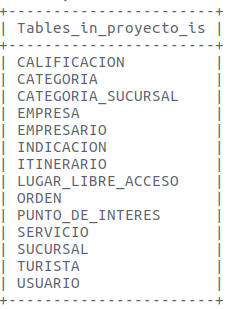
\includegraphics[scale=0.5]{captura1.png}\\ \includegraphics[scale=0.5]{"captura punto de interes.png}\\
\includegraphics[scale=0.5]{"captura empresario.png}
%%%%%%%%%%%%%%%%%%%%%%%%TESTING%%%%%%%%%%%%%%%%%%%%%%%%%%%%%%%%%%%%%%%
\subsection{Testing}
Hasta el momento hemos agregado información a tres tablas de la base de datos, USUARIO, TURISTA y EMPRESARIO, es decir contamos con información de personas que usarán la aplicación.\\\\
Los datos agregados son generados al azar automáticamente con la herramienta "\emph{generatedata}" encontrada online.\\\\
A continuación se muestra una captura de pantalla de la consola de mysql con la consulta que retorna aquellos usuarios turistas con edad entre 18 y 45 años.\\
\includegraphics[scale=0.7]{"captura consulta.jpg}
%%%%%%%%%%%%%%%%%%%%%%%%TRANSICION%%%%%%%%%%%%%%%%%%%%%%%%%%%%%%%%%
%\subsection{Transición}
%%%%%%%%%%%%%%%%%%%%%%%%%CONCLUSIONES%%%%%%%%%%%%%%%%%%%%%%%%%%%%%%%%%%
\section{Conclusiones}
Para la problemática planteada se propuso un sistema computacional que permita el fácil acceso a servicios turísticos en la provincia de Arauco cuya visualización se realizará a través de una aplicación móvil.\\\\
El diseño de la aplicación cuenta de varias etapas. En primera instancia generamos una lista de requisitos que debe cumplir la aplicación. Luego identificamos los actores involucrados y los casos de uso del sistema. Para poder crear la base de datos se llevó a cabo el diseño en un diagrama UML que posteriormente se pasó a modelo relacional. Con el modelo relacional terminado fuimos capaces de implementarlo usando MySQL. Hasta el momento hemos agregado datos de usuarios a la base de datos, por lo que para la próxima iteración deberemos poblar el resto de la base de datos.\\\\
Una vez que hayamos completado la fase de poblamiento de la base de datos, se procederá a comenzar el desarrollo propiamente tal de la aplicación, presentando finalmente un prototipo que servirá como demostración del producto y a la vez para realizar pruebas.
\end{document}